\section{Package Model}\begin{figure}[h!]
\begin{center}
	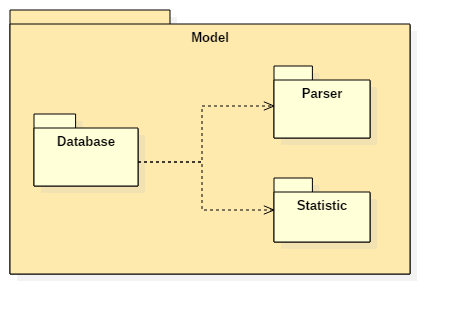
\includegraphics[scale=0.7]{../images/ModelPackage.png}
\end{center}
\end{figure}
\subsection{Model::Database}
\subsubsection{Model::Database::QuizManager}
\begin{itemize}
\item\textbf{Funzione del componente:} la classe permettera' l'inserimento, la lettura e la rimozione di questionari all'interno della collezione
\item\textbf{Relazioni d'uso con altre componenti:} ViewModel::Methods::QuestionMethods\\
\item\textbf{Metodi}:
\begin{itemize}
	\item\code{+ AddQuiz()}\\
	\textbf{Parametri}:
	\begin{itemize}
		\item\code{utente: string}\\
		\item\code{testo\_QML: string}\\
		\item\code{categoria: string}\\
	\end{itemize}
	\item\code{+ ModifyQuiz()}\\
	\textbf{Parametri}:
	\begin{itemize}
		\item\code{ID\_utente: int}\\
		\item\code{ID\_quiz: int}\\
		\item\code{Domande: string}\\
	\end{itemize}
	\item\code{+ RemoveQuiz()}\\
	\textbf{Parametri}:
	\begin{itemize}
		\item\code{ID\_utente: int}\\
		\item\code{ID\_quiz: int}\\
	\end{itemize}
\end{itemize}

\subsubsection{Model::Database::QuestionManager}
\begin{itemize}
\item\textbf{Funzione del componente:} la classe permettera' l'inserimento, la lettura e la rimozione di singoli quesiti all'interno della collezione
\item\textbf{Relazioni d'uso con altre componenti:} ViewModel::Methods::QuizMethods\\
\item\textbf{Metodi}:
	\begin{itemize}
		\item\code{+ AddQuestion()}\\
		\textbf{Parametri}:
			\begin{itemize}
				\item\code{utente: string}\\
				\item\code{testo\_QML: string}\\
				\item\code{categoria: string}\\
			\end{itemize}
		\item\code{+ ModifyQuestion()}\\
		\textbf{Parametri}:
			\begin{itemize}
				\item\code{ID\_utente: int}\\
				\item\code{ID\_quesito: int}\\
				\item\code{testo\_QML: string}\\
				\item\code{categoria: string}\\
			\end{itemize}
		\item\code{+ RemoveQuestion()}\\
		\textbf{Parametri}:
			\begin{itemize}
				\item\code{ID\_utente: int}\\
				\item\code{ID\_quesito: int}\\
			\end{itemize}
	\end{itemize}
\end{itemize}

\subsection{Model::Parser}
\subsubsection{Model::Parser::Parser}
\begin{itemize}
\item\textbf{Funzione del componente:} controlla che il testo fornito risulti corretto secondo la sintassi QML
\item\textbf{Relazioni d'uso con altre componenti:} QuestionManager\\
\item\textbf{Metodi}:
	\begin{itemize}
		\item\code{+ Check()}\\
		\textbf{Parametri}:
			\begin{itemize}
				\item\code{testo\_da\_controllare: string}\\
			\end{itemize}
	\end{itemize}
\end{itemize}

\subsection{Model::Statistics}
\subsubsection{Model::Statistics::Statistics}
\begin{itemize}
\item\textbf{Funzione del componente:} questa classe fornisce funzionalita' per il raccoglimento delle statistiche sulle prestazioni degli utenti del sistema
\item\textbf{Relazioni d'uso con altre componenti:} Nessuna\\
\item\textbf{Metodi}:
\begin{itemize}
	\item\code{+ UpdateQuestionStatitics()}\\
	\textbf{Parametri}:
	\begin{itemize}
		\item\code{ID\_quesito: int}\\
		\item\code{Corretta: bool}\\
	\end{itemize}
	\item\code{+ UpdateQuizStatitics()}\\
	\textbf{Parametri}:
	\begin{itemize}
		\item\code{ID\_quiz: int}\\
		\item\code{ID\_utente: int}\\
		\item\code{Risposte: Array}\\
	\end{itemize}
	\item\code{+ UpdateUserStatitics()}\\
	\textbf{Parametri}:
	\begin{itemize}
		\item\code{ID\_utente: int}\\
		\item\code{quesiti\_corretti: int}\\
		\item\code{quesiti\_totali\_quiz: int}\\
	\end{itemize}
\end{itemize}
\end{itemize}

\subsection{Model::Publishers}
\subsubsection{Model::Publishers::UserPublishers}
\begin{itemize}
\item\textbf{Funzione del componente:} questa classe fornisce funzionalita' per rendere pubblica la collezione degli utenti all'avvio del Sistema
\item\textbf{Relazioni d'uso con altre componenti:} Nessuna \\
\item\textbf{Metodi}:
	\begin{itemize}
		\item\code{+ PublishUser()}\\
	\end{itemize}
\end{itemize}

\subsubsection{Model::Publishers::QuizPublishers}
\begin{itemize}
\item\textbf{Funzione del componente:} questa classe fornisce funzionalita' per rendere pubblica la collezione dei quiz all'avvio del Sistema
\item\textbf{Relazioni d'uso con altre componenti:} Nessuna \\
\item\textbf{Metodi}:
	\begin{itemize}
		\item\code{+ PublishQuiz()}\\
	\end{itemize}
\end{itemize}

\subsubsection{Model::Publishers::QuestionPublishers}
\begin{itemize}
\item\textbf{Funzione del componente:} questa classe fornisce funzionalita' per rendere pubblica la collezione dei quesiti all'avvio del Sistema
\item\textbf{Relazioni d'uso con altre componenti:} Nessuna \\
\item\textbf{Metodi}:
	\begin{itemize}
		\item\code{+ PublishQuestion()}\\
	\end{itemize}
\end{itemize}